\chapter{METHODOLOGY}

This chapter describes how the research was designed and executed. It covers the overarching research paradigm, the requirements analysis process, the user-centred design methodology applied to the interface, the agile development approach, and the empirical evaluation protocol. The second half provides a detailed technical description of the AI pipeline architecture, including the actual prompt engineering strategy, the pattern matrix used for question type selection, and the Zod validation approach.

% ─────────────────────────────────────────────────────────────────────────────
\section{Overview}

\textbf{Research Design Paradigm.}

This research follows a \emph{design science} paradigm~\cite{sommerville2016}, appropriate for software engineering and information systems research where the primary contribution is a novel software artefact rather than a theoretical observation. The paradigm requires the artefact to be novel, to solve the identified problem effectively, and for its utility to be demonstrated through empirical evaluation.

The research is structured around two sequential phases:

\begin{enumerate}
  \item \textbf{Constructive phase.} User requirements are elicited from the target demographic. The system architecture is designed and implemented, including the frontend SPA, backend REST APIs, and the AI pipeline (transcript extraction, prompt formatting, LLM inference, and Zod validation).

  \item \textbf{Evaluative phase.} Once the platform reaches a stable, feature-complete state, a controlled comparative usability study measures it against the WordPress H5P workflow on three metrics: task completion rate, time-on-task, and SUS score.
\end{enumerate}

\textbf{Software Development Methodology.}

An \emph{agile} development methodology was used throughout the constructive phase, with iterative two-to-three week sprints each producing a testable increment~\cite{beck2001}. This approach was chosen specifically because the interaction between the AI pipeline, the H5P schema requirements, and the user experience could not be fully specified in advance. Critical usability constraints and technical edge cases only became apparent during active development and required immediate architectural changes.

% ─────────────────────────────────────────────────────────────────────────────
\section{User requirement analysis}
\label{sec:requirements}

\textbf{User Research and Elicitation.}

The first step was qualitative user research to understand the actual pain points of the target demographic. Semi-structured interviews with five instructors at HCMIU, from both technical and non-technical disciplines, consistently revealed four themes:
(1) The WordPress/H5P workflow feels completely disconnected from the actual teaching task;
(2) Instructors worry about losing their work when the browser reloads or a plugin times out mid-edit;
(3) Manual content creation---finding timestamps, typing questions, formatting distractors---takes more time than most instructors can spare;
(4) There is strong interest in AI-assisted question generation tied directly to the video's content.

A direct observation session, where a participant attempted to create a three-question interactive video with the baseline WordPress tool, confirmed the 45-to-60 minute completion time. The most common causes of task abandonment were losing track of the video position while filling out forms, and cryptic plugin error messages that gave no indication of what went wrong.


\begin{figure}[H]
  \centering
  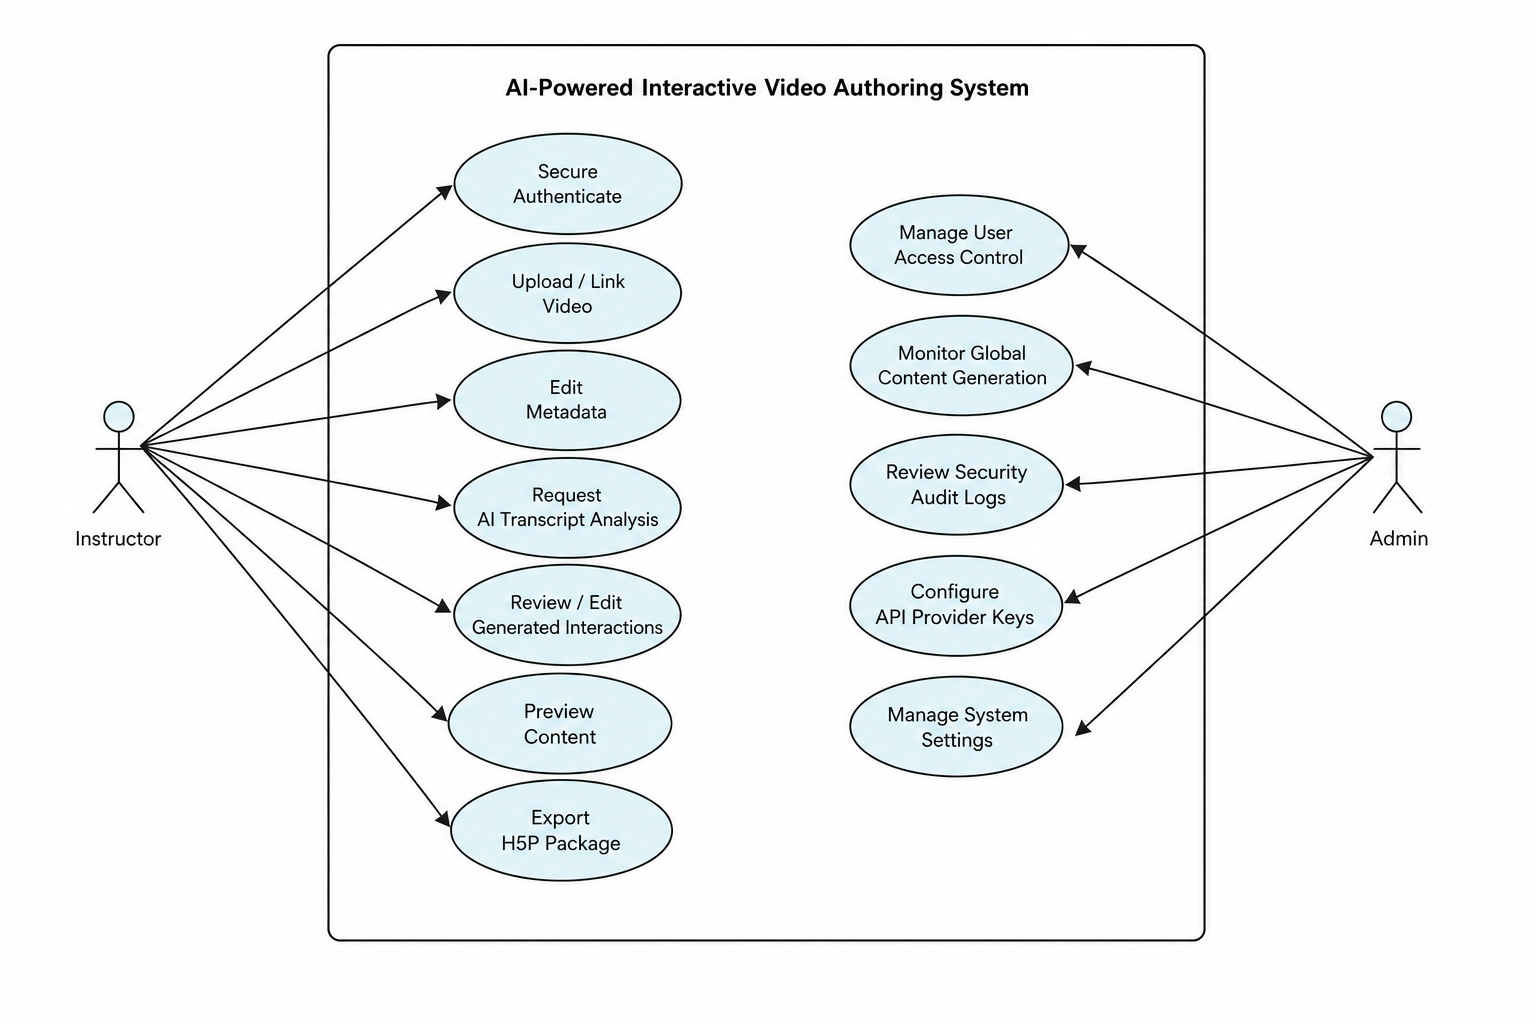
\includegraphics[width=0.85\linewidth,height=0.65\textheight,keepaspectratio]{images/Usecase.png}
  \caption{Use case diagram}
  \label{fig:usecase}
\end{figure}

\subsection{Functional and Non-Functional Requirements}

The interviews and observation session produced the following functional requirements:
\begin{itemize}
  \item \textbf{Authentication \& Access:} JWT-based stateless sessions, role-based access control, email verification.
  \item \textbf{Media Management:} Video file upload up to 500MB, YouTube URL import, timeline-based H5P editor, real-time content preview.
  \item \textbf{H5P Core Functionality:} Full support for six H5P interaction types, both manual and AI-assisted, with a one-click \texttt{.h5p} export.
  \item \textbf{AI Pipeline Integration:} Transcript extraction feeding an analysis pipeline that produces validated H5P JSON suggestions, delivered via Server-Sent Events (SSE) for real-time streaming.
  \item \textbf{Authoring Workflow:} Accept/reject/edit workflow for reviewing AI suggestions before injection into the H5P content database.
  \item \textbf{Administration:} Admin dashboards for user management, system monitoring, and an LTI 1.3 integration stub.
\end{itemize}

\textbf{Non-Functional Requirements.}

Table~\ref{tab:nonfunc_reqs} lists the quality and performance baselines the system must satisfy.

\begin{table}[H]
  \centering
  \begin{tabularx}{\linewidth}{l >{\raggedright\arraybackslash}p{3.0cm} X}
    \toprule
    \textbf{ID} & \textbf{Category} & \textbf{Requirement Definition} \\
    \midrule
    NFR-01 & Performance & All standard REST API responses must complete within 500\,ms under a load of 50 concurrent users. \\
    \addlinespace
    NFR-02 & Performance & Initial video upload processing (thumbnail/metadata) must complete within 30\,s for files $\leq 100$\,MB. \\
    \addlinespace
    NFR-03 & Security    & Passwords must be hashed using bcrypt with a cost factor of at least 12. \\
    \addlinespace
    NFR-04 & Security    & Authentication tokens must use stateless JWT, signed with HS256, expiring after 7 days. \\
    \addlinespace
    NFR-05 & Security    & All HTTP responses must enforce Helmet-generated security headers (CORS, CSP, XSS protection). \\
    \addlinespace
    NFR-06 & Security    & All API endpoints must validate input payloads using Zod schemas. \\
    \addlinespace
    NFR-07 & Reliability & The AI system must handle LLM failures gracefully, returning structured errors rather than crashing. \\
    \addlinespace
    NFR-08 & Usability   & The platform must achieve a minimum SUS score of 70. \\
    \addlinespace
    NFR-09 & Usability   & First-time task completion rate for creating an interactive video must exceed 80\%. \\
    \addlinespace
    NFR-10 & Compatibility & Exported \texttt{.h5p} packages must be valid for Moodle 4.x and Canvas LMS. \\
    \bottomrule
  \end{tabularx}
  \small
  \caption{Non-functional requirements driving system architecture}
  \label{tab:nonfunc_reqs}
\end{table}

% ─────────────────────────────────────────────────────────────────────────────
\section{System Design}
\label{sec:architecture}

\textbf{Architectural Overview and Topologies.}

The platform uses a three-tier architecture separating the presentation layer from business logic and data persistence~\cite{bass2012}.
The \emph{presentation tier} is a React 18 SPA built with Vite and Zustand for global state management.
The \emph{application tier} is an Express.js REST API on Node.js, responsible for all business logic, H5P library rendering, and AI pipeline routing.
The \emph{data tier} uses SQLite managed via Sequelize ORM, which provides fast local development with a clear migration path to PostgreSQL for larger deployments.

External dependencies are limited to: Groq API (primary cloud AI inference using \texttt{llama-3.3-70b-versatile}), Ollama (local offline AI fallback), and the YouTube Data API. All H5P processing runs within the local server process.

\begin{figure}[H]
  \centering
  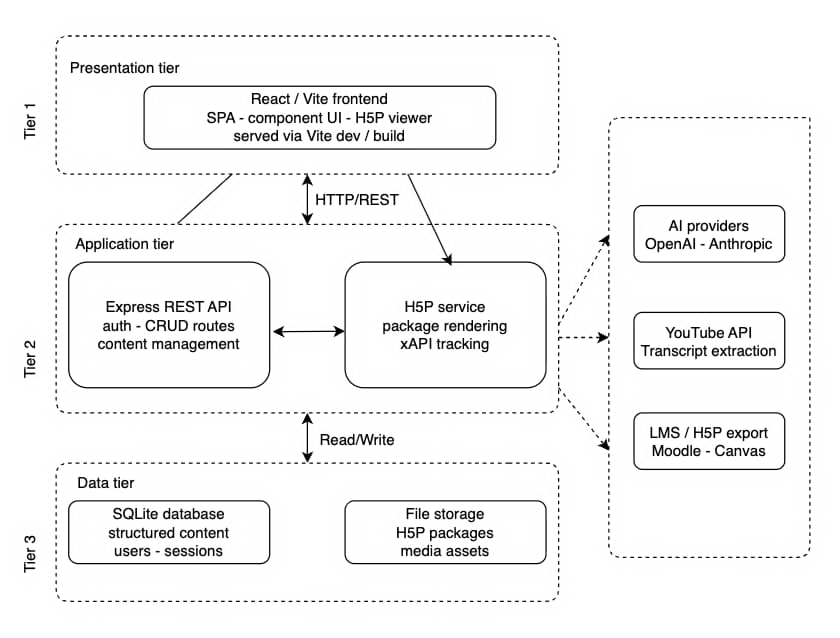
\includegraphics[width=0.85\linewidth,height=0.65\textheight,keepaspectratio]{images/Three-tỉer system.jpeg}
  \caption{Three-tier system architecture}
  \label{fig:architecture}
\end{figure}

The design goals were: strict separation of concerns via a versioned REST API; AI-provider independence through a uniform JSON output shape regardless of the underlying LLM; H5P library isolation using the Lumi headless server package; and a stateless backend using JWT tokens for horizontal scaling.

\textbf{API Route Structure and Controller Logic.}

The REST API is organized under the \texttt{/api/v1/} prefix, with authentication and rate-limiting middleware at the router level. Table~\ref{tab:api_routes} lists the primary functional route groups.

\begin{table}[H]
  \centering
  \begin{tabularx}{\linewidth}{
    >{\raggedright\arraybackslash}p{5.0cm}
    >{\raggedright\arraybackslash}p{1.5cm}
    X
  }
    \toprule
    \textbf{Prefix} & \textbf{Methods} & \textbf{Responsibility} \\
    \midrule
    \path{/api/auth} & POST & Registration, login, bcrypt password verification, JWT issuance and refresh. \\
    \addlinespace
    \path{/api/videos} & GET, POST, PUT, DELETE & Video upload, YouTube URL validation, thumbnail generation, metadata CRUD. \\
    \addlinespace
    \path{/api/h5p} & GET, POST, DELETE & H5P parameter CRUD, zip package generation, iframe rendering. \\
    \addlinespace
    \path{/api/ai/analyze} & POST & Synchronous transcript analysis returning a full JSON payload. \\
    \addlinespace
    \path{/api/ai/analyze-stream} & POST & Asynchronous transcript analysis; questions streamed via SSE. \\
    \addlinespace
    \path{/api/ai/inject} & POST & Validates and injects accepted AI suggestions into the H5P content store. \\
    \addlinespace
    \path{/api/transcript} & POST & YouTube caption extraction, VTT parsing, and segment normalization. \\
    \addlinespace
    \path{/api/admin} & GET, POST, PUT & User management and audit logs (Admin RBAC only). \\
    \addlinespace
    \path{/api/lti} & GET, POST & OIDC handshake for LTI 1.3 deep-linking. \\
    \bottomrule
  \end{tabularx}
   \small
  \caption{REST API route groups and functional responsibilities}
  \label{tab:api_routes}
\end{table}

% ─────────────────────────────────────────────────────────────────────────────
\section{AI Pipeline Architecture}

The AI pipeline is the most technically complex part of the platform. Its job is to transform a raw, timestamped video transcript into a validated, Bloom's taxonomy-labelled list of H5P interaction JSON configurations. The transformation happens through a five-stage process. Figure~\ref{fig:ai_pipeline} shows the overall data flow, and Figure~\ref{fig:seq_ai} shows the detailed sequence diagram including the SSE streaming path.

\begin{figure}[H]
  \centering
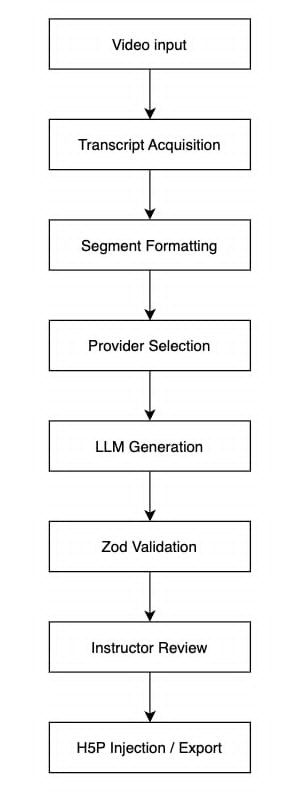
\includegraphics[width=0.85\linewidth,height=0.65\textheight,keepaspectratio]{images/AI Pipeline.jpeg}
  \caption{AI pipeline flowchart}
  \label{fig:ai_pipeline}
\end{figure}

\begin{figure}[H]
  \centering
 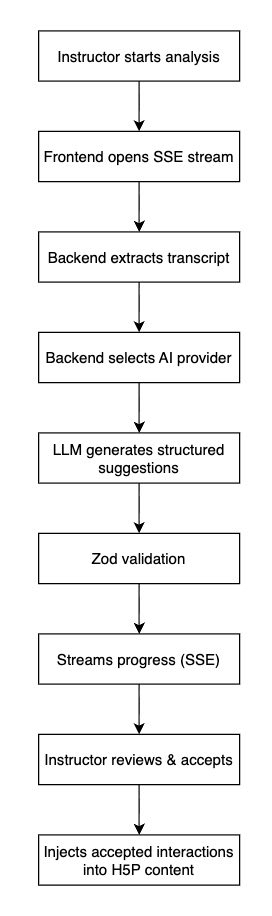
\includegraphics[width=0.85\linewidth,height=0.65\textheight,keepaspectratio]{images/AI asisted question generation.jpeg}
  \caption{AI-assisted question generation sequence diagram}
  \label{fig:seq_ai}
\end{figure}

\textbf{Stage 1: Transcript Acquisition and Normalization.}

Transcript acquisition is handled by \texttt{transcriptExtraction.js}, which supports three source mechanisms:

\begin{enumerate}
  \item \textbf{YouTube Automatic/Manual Captions.} The \texttt{youtube-transcript} package fetches timestamped XML caption segments directly from the YouTube API using the video's 11-character ID. These are parsed and normalized into a standard three-field JavaScript object: start time, end time (both in seconds), and text string.
  \item \textbf{Uploaded WebVTT Caption Files.} Instructors can upload a \texttt{.vtt} or \texttt{.srt} file alongside their video. A regex-based parser extracts timing cues and text, normalizing them into the same format.
  \item \textbf{Whisper Audio Transcription.} For uploaded videos without captions, the service invokes \texttt{faster-whisper} via a Python subprocess, passing the video file path and requesting transcription. The resulting JSON transcript is normalized into the standard segment format. Whisper availability is checked at server startup and reported via \texttt{GET}~\path{/api/ai/status}~\cite{radford2023}.
\end{enumerate}

All three sources produce the same \texttt{TranscriptSegment[]} data structure, ensuring the downstream AI stage is completely decoupled from the extraction logic.

\textbf{Stage 2: Segment Formatting and Smart Selection.}

The \texttt{formatSegmentsForPrompt()} function in \texttt{aiService.js} converts the normalized segment array into a compact, line-delimited string for the LLM prompt. Each line uses the format:

\begin{verbatim}
[330s-345s] Photosynthesis converts light energy into chemical energy.
\end{verbatim}

The compact \texttt{[Xs-Ys]} timestamp notation (e.g.\ \texttt{[330s-345s]}) saves roughly 22 characters per line compared to a verbose human-readable format, reducing the total token count by approximately 600 tokens for a 100-segment transcript. The raw-second values are used directly in the JSON output so the model never needs to perform time arithmetic, which eliminates a common source of timestamp hallucination~\cite{white2023}.

Rather than uniform sub-sampling, the function applies a \emph{smart selection} strategy. The video timeline is divided into equal windows, and from each window the segment with the highest information score is retained. Segments that begin with topic-transition markers (e.g.\ ``Now'', ``Next'', ``Finally'', ``To summarise'') receive a score bonus, as do segments containing questions. Short filler segments (fewer than four words) receive a penalty. This ensures the model receives denser, more useful context in fewer tokens, preserving topic boundaries more faithfully than uniform sub-sampling across the same token budget. For a 10-minute video with 300 segments, the function typically selects 80--100 high-value segments.

\textbf{Stage 3: Two-Step AI Prompt Engineering and Question-Type Assignment}
\label{sec:stage3}

The core AI system prompt, defined as the constant \texttt{AI\_SYSTEM\_PROMPT} in \texttt{aiService.js}, implements a two-step \emph{output automater} prompting pattern~\cite{white2023}. The key idea is to separate high-level topic discovery from the mechanical task of generating JSON. By constraining what the model needs to do at each step, output consistency improves significantly.

\subsubsection{Step 1 --- Hierarchical Topic Segmentation}

In the first step, the model receives the formatted transcript and is told to act as an instructional designer. It must produce a hierarchical topic outline covering the full video. The prompt specifies that a well-structured lecture will typically produce 4--10 topics depending on content density, and explicitly instructs the model not to inflate the count by artificially splitting unified concepts.

Topic boundaries are detected using specific linguistic markers. The system prompt lists English markers (``Next'', ``Moving on'', ``Now let's'', ``Another'', ``Finally'') and Vietnamese markers (``Tiếp theo'', ``Bây giờ'', ``Chuyển sang'', ``Tóm lại'') explicitly, rather than relying on the model's general knowledge. This specificity helps the model apply consistent segmentation logic regardless of input language.

The timestamp rules are stated explicitly. The model is instructed to read each line's \texttt{[Xs-Ys]} prefix, use the raw second integers directly as \texttt{start}/\texttt{end} fields in its JSON output, never invent or estimate timestamps, ensure topics do not overlap, and cover the full video from first to last segment. This level of specificity is deliberate. General instructions such as ``use the correct timestamp'' leave too much ambiguity, and models frequently produce timestamps that do not correspond to any value in the input without explicit rules~\cite{white2023}.

\subsubsection{Step 2 --- Deterministic Question Generation via Pattern Matrix}

The second step uses a rigid pattern matrix to force the model to map each topic's content characteristics to exactly one of the six supported H5P interaction types. The model is instructed to generate exactly one question per topic following this mapping: a topic that introduces a definition maps to \texttt{FillBlanks}; a binary fact or principle maps to \texttt{TrueFalse}; a comparison, list, or process maps to \texttt{MultiChoice}; an ordered sequence of steps maps to \texttt{DragText}; and a passage with multiple key terms maps to \texttt{MarkWords}. One additional topic titled ``Video Recap'' is appended at the end of the video with a \texttt{Matching} question covering 4--5 concept pairs drawn from the entire video.

Table~\ref{tab:pattern_matrix} shows the complete mapping between content characteristics, pedagogical knowledge focus, H5P type, and required JSON fields.

\begin{table}[H]
  \centering
  \begin{tabularx}{\linewidth}{
    >{\raggedright\arraybackslash}p{2.8cm}
    >{\raggedright\arraybackslash}p{2.2cm}
    >{\raggedright\arraybackslash}p{2.4cm}
    >{\raggedright\arraybackslash}X
    >{\raggedright\arraybackslash}X}
    \toprule
    \textbf{Content type} & \textbf{Bloom's level} & \textbf{H5P type} & \textbf{Generation rule} & \textbf{Key JSON fields} \\
    \midrule
    Definition / technical term  & Remember / Understand  & \texttt{FillBlanks}  & Ask for the key term in context & \texttt{fillText} (target wrapped in \texttt{*asterisks*}) \\
    \addlinespace
    Binary fact / absolute rule  & Remember  & \texttt{TrueFalse}   & Turn the statement into a verifiable claim & \texttt{question}, \texttt{correct} (boolean) \\
    \addlinespace
    List / comparison / process  & Understand / Analyze  & \texttt{MultiChoice} & Four options, one correct, three plausible distractors & \texttt{question}, \texttt{answers[4]} \\
    \addlinespace
    Sequence / ordered procedure & Apply  & \texttt{DragText}    & Convert ordered steps into draggable phrases & \texttt{taskDescription}, \texttt{textField} \\
    \addlinespace
    Vocabulary / key terms       & Remember / Understand  & \texttt{MarkWords}   & Identify key terms in a short passage & \texttt{taskDescription}, \texttt{textField} \\
    \addlinespace
    Cross-topic review recap     & Analyze / Evaluate  & \texttt{Matching}    & Pair overarching concepts with definitions & \texttt{taskDescription}, \texttt{pairs[]} \\
    \bottomrule
  \end{tabularx}
  \small
  \caption{H5P interaction types and their AI-guided selection rules}
  \label{tab:pattern_matrix}
\end{table}

The pattern matrix reduces the model's output space from an open-ended question format down to a choice among six templates with precisely defined JSON schemas. Each type has different required fields. A \texttt{FillBlanks} question needs a \texttt{fillText} string with the answer term wrapped in asterisks (\texttt{*term*}). A \texttt{MultiChoice} question needs a \texttt{question} string and an \texttt{answers} array of exactly four objects, each with \texttt{text} and \texttt{correct} fields. A \texttt{Matching} question needs a \texttt{pairs} array of \texttt{\{prompt, answer\}} objects. The prompt provides a worked example for each type to make these schema differences concrete.

The reasoning behind this matrix deserves explanation. The choice between question types is not arbitrary---it follows from how the content is structured:

\begin{itemize}
  \item \textbf{Definitions} are best tested with fill-in-the-blanks because the task is to retrieve a specific term, not choose among alternatives. Providing the surrounding context with a blank maintains the meaning of the statement.
  \item \textbf{Binary facts} (things that are always true, always false, or universally applicable) are best tested with true/false because the learner's decision is binary.
  \item \textbf{Comparisons and lists} work well as multiple choice because the distinguishing features of each item can serve as answer options, and wrong options can be drawn from other items in the same category.
  \item \textbf{Sequences} require the learner to recall order, which drag-text supports naturally by having the learner reconstruct the sequence rather than recognize it.
  \item \textbf{Vocabulary identification} works differently from definition recall---the learner recognizes which terms in a passage are technically important, which is what mark-the-words tests.
  \item \textbf{Recap} at the end of the video pairs key concepts introduced throughout the lecture with their definitions---the matching type's primary use case.
\end{itemize}

\subsubsection{Resilient Provider Selection and Fallback Specification}

The AI generation pipeline uses a three-tier fallback chain. All provider attempts happen \emph{before} SSE headers are written to the HTTP response. Once headers are committed, switching providers is impossible, so any mid-stream failure is delivered as a structured SSE error event rather than a server crash.

Table~\ref{tab:fallback} summarises the complete cascade, from primary model to graceful failure.

\begin{table}[H]
  \centering
  \small
  \begin{tabularx}{\linewidth}{
    >{\centering\arraybackslash}p{0.8cm}
    >{\raggedright\arraybackslash}p{4.8cm}
    >{\raggedright\arraybackslash}X
    >{\raggedright\arraybackslash}p{3.5cm}}
    \toprule
    \textbf{Tier} & \textbf{Provider / Model} & \textbf{Trigger Condition} & \textbf{Outcome} \\
    \midrule
    1 & Groq --- \textit{llama-3.3-70b-versatile} & Normal operation; key present; within rate limits & Fast generation, 5--10 s; 100 segs; 4\,200 tokens \\
    \addlinespace
    2 & Groq --- \textit{llama-3.1-8b-instant} & HTTP 429 (rate limit) or HTTP 413 (payload too large) on Tier~1 & Downgraded capacity; 50 segs; 2\,500 tokens; slightly lower quality \\
    \addlinespace
    3 & Local Ollama --- \textit{llama3.1:8b} & Any Groq failure before SSE headers: invalid/missing key (401), all Groq models rate-limited, or network unreachable & No API key; 30--90 s; no rate limit \\
    \addlinespace
    4 & None & Ollama also unreachable & Structured SSE error event sent to browser; no server crash (NFR-07) \\
    \bottomrule
  \end{tabularx}
  \caption{AI provider fallback cascade: trigger conditions and outcomes}
  \label{tab:fallback}
\end{table}

The critical design constraint is that \emph{provider selection must complete before the first SSE byte is sent}. The \texttt{runGroqAnalysis()} function therefore initiates the Groq streaming request synchronously before writing any response headers. If the SDK throws at that point---on authentication failure, quota exhaustion, or network error---the exception propagates to the caller, which can cleanly attempt Tier 3. If Groq successfully opens the stream and then fails mid-stream (a rare network drop after headers are already committed), there is no recovery path, and the partial content is discarded via a terminal error event.

Regardless of which tier handles the request, the React frontend receives an identical SSE event stream with the same type-safe topic and question structure. The UI behaviour is provider-transparent.

\pagebreak
\textbf{Stage 4: Zod Validation and Data Enrichment}

After receiving the raw string output from the LLM, the backend parses it with \texttt{JSON.parse()} and immediately runs it through Zod schema validation. The schemas are defined in \texttt{aiService.js}:

\noindent\begin{minipage}{\linewidth}
\begin{lstlisting}[language=JavaScript,caption={Zod schemas for validating AI output}]
const QuestionSchema = z.object({
  type: z.enum([
    'MultiChoice', 'TrueFalse', 'FillBlanks',
    'DragText', 'MarkWords', 'Matching'
  ]),
  question:        z.string().min(1).optional(),
  answers:         z.array(z.object({
    text: z.string().min(1), correct: z.boolean()
  })).optional(),
  correct:         z.boolean().optional(),
  fillText:        z.string().min(1).optional(),
  taskDescription: z.string().min(1).optional(),
  textField:       z.string().min(1).optional(),
  pairs: z.array(z.object({
    prompt: z.string().min(1), answer: z.string().min(1)
  })).optional(),
  feedback: z.object({ correct: z.string(), incorrect: z.string() })
    .catch({ correct: 'Correct!', incorrect: 'Please review.' }),
});
const TopicSchema = z.object({
  title:    z.string(),
  start:    z.number().catch(0),
  end:      z.number().catch(0),
  question: QuestionSchema.catch(undefined).optional(),
});
const ResponseSchema = z.object({ topics: z.array(TopicSchema) });
\end{lstlisting}
\end{minipage}

The \texttt{.catch()} calls on the \texttt{start} and \texttt{end} fields and the \texttt{feedback} object are worth noting. Rather than throwing a validation error when those fields are missing or malformed, Zod replaces them with defaults. A topic node that fails timestamp validation doesn't cause the entire response to be discarded---it gets a fallback timestamp of 0 and the instructor can adjust it manually. The goal is to maximize the number of usable suggestions recovered from a partially malformed LLM response. A 15-second generation that produces five out of six valid suggestions is far more useful than one that throws a 500 error.

Valid topics are enriched with a system-generated content ID and the resolved H5P library identifier. Table~\ref{tab:h5p_type_map} shows the mapping from question type to library identifier. These identifiers are what the H5P player uses to load the correct JavaScript runtime; an incorrect identifier causes the content to render nothing.

\begin{table}[H]
  \centering
  \begin{tabular}{ll}
    \toprule
    \textbf{Question type} & \textbf{H5P library identifier} \\
    \midrule
    \texttt{MultiChoice} & \texttt{H5P.MultiChoice 1.16} \\
    \texttt{TrueFalse}   & \texttt{H5P.TrueFalse 1.6}   \\
    \texttt{FillBlanks}  & \texttt{H5P.Blanks 1.14}     \\
    \texttt{DragText}    & \texttt{H5P.DragText 1.10}   \\
    \texttt{MarkWords}   & \texttt{H5P.MarkTheWords 1.9}\\
    \texttt{Matching}    & \texttt{H5P.Matching 1.0}    \\
    \bottomrule
  \end{tabular}
  \caption{Question type to H5P library identifier mapping}
  \label{tab:h5p_type_map}
\end{table}

\textbf{Stage 5: Instructor UI Review and Database Injection.}

Once AI generation completes and validated suggestions are streamed to the UI, the instructor reviews them, makes any necessary edits, and selects which questions to keep. A \texttt{POST} request to \texttt{/api/ai/inject} sends the accepted suggestions to the \texttt{aiInjectionService.js} backend module, which writes them to the database. This process is described in detail in Chapter~4.
